%----------------------------------------------------------------------------------------
%----------------------------------------------------------------------------------------
%       CHAPTER 00
%----------------------------------------------------------------------------------------
%----------------------------------------------------------------------------------------

\cleardoublepage

\chapterimage{muffin_planet.jpg} % Chapter heading image

\setcounter{chapter}{-1}
\chapter{Installation, Configuration, Basic Usage}\label{ch:0}

\hfill \break

\vspace{16mm}

\noindent Stuff to keep in mind:

\vspace{2mm}

\begin{itemize}
\item \textbf{(cGENIE.)cookie} is a \uline{model}. Models ARE NOT the ‘real World’. (Don’t get confused!)
\item The  low resolution (for a 3-D ocean circulation model) of the \textbf{cookie} model limits its applicability for very short time-scale problems.\ In configurations not incorporating the \textbf{PLASIM} atmospheric GCM component, there are no atmospheric dynamics or inter-annual variability in the coupled ocean-atmosphere system.
\item \textbf{cookie} is best thought of as a ‘discovery and exploring’ tool for learning how the Earth system has functioned in the past rather than a detailed ‘simulation’ tool for the future.
\item It is possible to have fun.
\end{itemize}

%------------------------------------------------
\newpage
%------------------------------------------------

\section{Before anything else …}

%------------------------------------------------

\subsection*{ReadMe}

Some warnings and reminders in this manual are repeated over and over and over and … over again.
Some warnings and reminders are repeated over and over and over and … over again.
This is because you will forget immediately each time! ;)
\\\textbf{!}\footnote{\textbf{Also read footnotes please.}}

%------------------------------------------------

\subsection*{Software version naming conventions}

You will be using the current version of the cGENIE Earth system model, code-named ‘\textbf{cookie}’ (if \textbf{Apple} can have ‘Leopard’, ‘Lion’ etc., I can have a baked goods version naming convention). The documentation may not be fully consistent in this respect … and you may need to translate occurrences of e.g. a directory named ‘\texttt{cgenie}’ to ‘\texttt{cgenie.cookie}’. For brevity, the \textbf{cGENIE.cookie} model will be referenced by just ‘\textbf{cookie}’.

%------------------------------------------------

\subsection*{linux ...}

The \textbf{(cGENIE.)cookie} model currently naively compiles and runs under \textbf{linux}\footnote{For some of you, the mechanics of running the model will be about as much fun as sticking your tongue in an electrical outlet (a popular hobby in England). (However, if you are an experienced linux/unix/tongue-in-electrical-socket user, you can skip onto the next Section and save yourself an entire 15 seconds of reading words.)} (e.g. distributions such as \textbf{Ubuntu}) and unix-like operating systems (such as \textbf{macOS}). \textbf{cookie} (like most climate models) is configured and accessed (aka ‘run') at the ‘command line’ of the linux (or \textbf{macOS} equivalent, which is unix-like) operating system. The command line is a place where you type text and when you press \small\textsf{Return}\normalsize, something (hopefully, good!) happens. Typically the stuff you type started with a ‘command’ word, and often followed by one or more options and parameters. The command word and any options / parameters MUST be separated by SPACEs.

The start of each line of the command line is indicated with something like: \texttt{\$}. The \texttt{\$} is called the ‘prompt’ and is ... prompting you to type some input (commands, Tweets, swear words, etc.). See – the computer is just sat there waiting for you to command it to go do something (stupid?). Typically, you will also be informed (reminded) of the user-name, computer name, and current directory, e.g.:

\vspace{-2mm}
\begin{verbatim}
[username@host ~]$
\end{verbatim}
\vspace{-2mm}

\noindent which is in this example is user ‘\texttt{username}’ (yours will be different!) on computer name ‘\texttt{host}’\footnote{Sprout the cat will eventually appear under ‘cat-of-the-day’ on my home-page if you press \textsf{F5} enough times – all my computing clusters are named after my cats …} and the current directory is the ‘home’ directory -- represented by the \texttt{\~} symbol. If, for example, you were instead currently in the \texttt{myfolder} directory, you would see at the command prompt something like:

\vspace{-2mm}
\begin{verbatim}
[username@host myfolder]$
\end{verbatim}
\vspace{-2mm}

If you are not or not very familiar with the linux/unix command line, such as how to navigate up and down the directory tree and to display the contents of the current directory you are in – for a brief summary of some basic/useful \textbf{linux} commands and usage -- see the linux HOW-TO Section towards the back of the book.

NOTE: BE VERY CAREFUL that spaces are not missed out when typing out example lines. Also be careful not to confuse the number one (\texttt{1}) for the letter 'el' (\texttt{l}). Mis-spelling/typing is generally the most likely reason for things not working.

NOTE-the-second: If you find yourself terminally bored typing in long long instructions lines, you may be tempted to simply copy-paste from the cookie manual PDF to the command line, This can work, but firstly be aware that trying to copy-paste multiple lines at once is doomed to failure -- copy-paste the first line and then following that add the second (or subsequent) line.
Also note that the inverted comma symbol in the PDF is not the same inverted comma symbol that linux is expecting ... You should also make liberal use of the up arrow key that bring back the previously entered command (keep pressing the key for progressively older commands). For instance, a mistake in a command line can be corrected by bringing back the offending line and using the left/right arrows to navigate through the characters and correct any mistake.

NOTE-the-third: In places, instructions may be given for specific programs and computer platforms and hence may differ slightly from the software reality in front of you. Use your judgement in translating such instructions. Many other alternative software choices exist for editing files or viewing results, as are other ways of configuring software and file editing/transferring methodologies. Do what suits you best – you can view such instructions where they occur, as  more representing an example methodology rather than a literal interpretation of the Constitution.

%------------------------------------------------

\subsection*{Required computer hardware/software}

For running \textbf{cupcake}, your options are:

\begin{enumerate}[noitemsep]

\vspace{1mm}
\item \textbf{Remotely}
\\To do this, you will need an account on a linux-based server or cluster. You can use any platform (\textbf{linux}, \textbf{macOS}, \textbf{Windoz}, as well as \textbf{iOS} and \textbf{Android} (which is based on \textbf{linux} in any case)) to connect to the cluster. You will need the following software on your local machine:
\vspace{1mm}
\begin{enumerate}[noitemsep]
\setlength{\itemindent}{.2in}
\item A terminal (‘shell’) window. This is no problem for \textbf{linux} and \textbf{Mac} users (you already have one built in). For \textbf{Windows}, either download a simple (and old) \textbf{SSH} client (ssh-client) from my website\footnote{http://www.seao2.info//cgenie/software/ssh-client.exe} or you can get hold of e.g. \textbf{PuTTY} (http://www.putty.org/).
\item A sftp (secure file transfer) client for convenience (i.e. dragging and dropping files between local and remote computers, and opening files directly on the remote computer cluster). If you have installed ssh-client (\textbf{Windows}, above) then a sftp client is already included as part of this software. If using \textbf{PuTTY} (\textbf{Windows}) you might try downloading \textbf{WinSCP} (http://winscp.net/eng/index.php). For \textbf{macOS}, you can connect to the server through the \textbf{Terminal}, but some sftp software for viewing/navigating server file structure include: \textbf{FileZilla} (recommended), \textbf{Cyberduck}, \textbf{TextWrangler}. For linux, maybe \textbf{FileZilla}.
\end{enumerate}

\vspace{1mm}
\item \textbf{Locally}
\\It is  possible to install and run the ‘\textbf{(cGENIE.)cookie}’ Earth system model either on a linux box (e.g. \textbf{Ubuntu}) or on a \textbf{Mac} \footnote{Sets of detailed installation instructions are available in the HOW-TO section of this manual.}\footnote{It is also possible to run \textbf{cookie} under \textbf{Windows}.}. At a minimum, you will need:
\vspace{1mm}
\begin{enumerate}[noitemsep]
\setlength{\itemindent}{.2in}
\item A FORTRAN (f90 and f77 combatable) compiler of some sort.
\\This may come with the operating system as standard, possibly \textbf{gfortran}.
\item A \textbf{git} client.
\\If not standard, this is relatively easy to add and install.
\item Compiled \textbf{netCDF} libraries (not so much fun ...).
\end{enumerate}
\vspace{1mm}
To edit files and visualize results, you will need some specific software. The exact software will depend on your operating system, but essential are:
\vspace{1mm}
\begin{enumerate}[noitemsep]
\setlength{\itemindent}{.2in}
\item A viewer for netCDF format spatial data. A \textbf{Java} viewer called \textbf{Panoply} is provided by NCAR for all platforms – http://www.giss.nasa.gov/tools/panoply/
(Note that you will need \textbf{Java} installed!) (Or alternatively: \textbf{MATLAB}, \textbf{python}, etc..)
\item  A simple text editor, except not the rubbish default \textbf{Windows} one – you need one that can display \textbf{unix} ASCII text without screwing it up. Options for \textbf{Windows} users are:
\textbf{notepad++} (https://notepad-plus-plus.org/)
\textbf{SciTE} (https://www.scintilla.org/SciTE.html)
(\textbf{linux} and \textbf{Mac} users need no special/different editor compared with your standard editor – everything will display just fine). You can also use \textbf{linux} command line based editors such as \textbf{vi}.
\end{enumerate}
\vspace{1mm}

\end{enumerate}
\vspace{1mm}

%------------------------------------------------

\subsection*{File editors ...}

You will need to edit text-based configuration files, possibly in installing and configuring \textbf{cookie}, but definitely in configuring model experiments. So now might be a good time to check that you can use the/an editor! (You will also be using the same editor to view some of the model output.)

You have two alternative options for editing and viewing text files, depending on whether you are a \textbf{unix} nerd with no life, or prefer anything to do with computers to be wrapped in cotton wool and covered with dollops of treacle.
EITHER: Use the linux \textbf{vi} (/\textbf{vim}) application (or similar e.g. \textbf{emacs}) if you are familiar with it. I think that this pretty much sucks as a text editor and life is far too short and brutal if you don't like this sort of thing … OR ... use a suitable linux-friendly text editor (NOT \textbf{Micro\$oft} \textbf{Notepad}) in conjunction with the \textbf{Secure File Transfer Client}. For example: \textbf{SciTE} (http://www.scintilla.org/SciTE.html) is suitable, or \textbf{Notepad++}.

If you fiddle about with the settings under Options/Preferences in the \textbf{WinSCP} program and apply a little common sense, it should be possible to configure things so that you can simply double-click on a file in the remote (right-hand) window panel and it will open like magic (almost)! Saving the file after editing) should then result in the file being saved back to the cluster. Or you can select Edit With (and then \textbf{SciTE}) from right-mouse-button-clicking on the filename. Or ... a crude but workable approach is to use an sftp client to drag the file to your local machine (assuming \textbf{cookie} is installed remotely), edit it there, and then drag it back again.\footnote{Note that care still has to be taken to avoid certain \textbf{Microsoft} text editing programs under \textbf{Windoz}.)}

%------------------------------------------------
\vspace{1mm}\noindent\rule{4cm}{0.5pt}\vspace{2mm}
%------------------------------------------------

%------------------------------------------------
\newpage
%------------------------------------------------

\subsection*{Model documentation in general}

This (the \textbf{cookie} manual), and additional documentation (of varying degrees of up-to-date-ness) can be found:

\vspace{1mm}
\begin{enumerate}[noitemsep]
\setlength{\itemindent}{.2in}
\item On \href{https://github.com/genie-model/cookiedoc}{GitHub}.
\\The \textbf{latex} source for the documentation lives here, allowing you to compile the most up-to-date PDF document. And ... make changes yourself and have them incorporated into the official documentation\footnote{First clone the \textbf{git} repository. Make changes. Commit them locally. Make a 'pull request' ...}.
\\However, note that you will have to compile the latex source yourself to create a PDF ...
\item On my \href{http://www.seao2.info/mymuffin.html}{website}.
\\Here you can find compiled PDF versions of the documentation ... but it could be a little out of date (the up-to-date latex sources lives on \textbf{GitHub}).
\end{enumerate}

%------------------------------------------------

\subsection*{This document in particular}

The instructions  may not be entirely bug-free -– use your judgment.

%------------------------------------------------

\subsection*{Go!}

OK – now we are ready to start …

%------------------------------------------------
\newpage
%------------------------------------------------

\section{Starting (dozing?) off …}

You are going to be installing the model from scratch – why? Why not? It will be a happy character-building experience for you ... trust me ...

%------------------------------------------------

\subsection{Logging in!}

In running \textbf{cookie} locally -- log into your \textbf{linux}/\textbf{macOS} box (and skip on to the next section)! \footnote{If you fail at this step, you'll have to take up box-modelling instead.}

\noindent Or ... and much more likely to be the case -- if you are running \textbf{cookie} \uline{remotely} (e.g. via a user account on a computing cluster or server), then log into the remote server or cluster account using a 'suitable terminal program'\footnote{It very much depends on what software you are using. Provided are instructions for some \uline{examples}, but only examples, and your reality may be rather different.}:

\begin{itemize}
\vspace{1mm}
\item If logging in via a \textbf{linux}/\textbf{macOS} box, open the terminal/shell window and simply SSH in\footnote{If your current directory looks something like this: \texttt{[username@clustername \(\sim\)]\$}
then you are probably already logged in! Otherwise, it will look like: \texttt{username@localcomputername:\(\sim\)\$}}, e.g.

\vspace{-1mm}
\begin{verbatim}
$ ssh username@clustername
\end{verbatim}
\vspace{-1mm}

where \texttt{clustername}, the cluster (or remote server) name(!) might, for example, be
\\\texttt{catname.ucr.edu}, and enter your  account password (and tell it whether or not you want this password stored, if asked).
\vspace{1mm}
\\\textbf{IMPORTANT!} -- When you type in a password in \textbf{linux}, NOTHING appears on the screen, not even \texttt{********} as in common on \textbf{Windoz}. As you type (the password), characters are being entered ... you just cannot see them. Don't panic -- just type in the password (even if you cannot see characters appearing) and hit \textsf{\scriptsize Enter}.

\vspace{1mm}
\item On a \textbf{Windoz} machine – first start the \textbf{WinSCP} program (an sftp file transfer client). Under \textsf{\footnotesize Host Name}, enter the remote server or cluster name (e.g. \texttt{catname.ucr.edu}):
\\The \textsf{\footnotesize Port number} should be set to \textsf{\footnotesize 22} (except for \texttt{sterling.ucr.edu}). Enter your computing cluster user-name on the line below this (‘\textsf{\footnotesize User Name}’) and then the \textsf{\footnotesize Password}. Click on \textsf{\footnotesize Login}.
\\You will also need a terminal window. This can be opened by clicking on the ‘\textsf{\footnotesize Open session in PuTTY}’ icon on the top icon row, or pressing \textsf{\footnotesize Ctrl+P}. \\You should now have TWO windows open – a ‘shell’ window (lines of text on an otherwise blank screen) and a file manager (transfer) window. Ensure that you have both these before moving on. It is recommended that you maximize both these windows to full screen. (But no-one will die horribly for not doing so. Probably ...).
\\ You can also log in directly from the shell/terminal window e.g. \textbf{PuTTY} first (rather than first opening an sftp connection first).
 You will sill have to open an sftp connection for file transfer.
\end{itemize}

\vspace{1mm}
Note that the cluster you access may not use the standard 'port' number of \textsf{\footnotesize 22}. If your computer uses a different port number -- in the login window of your sftp client, simply change the number in the \textsf{\footnotesize Port} box, or if you are using the command line, you will need to type:
\vspace{-1mm}
\begin{verbatim}
$ ssh -p xxxxx username@clustername
\end{verbatim}
\vspace{-1mm}
where \textsf{\footnotesize xxxxx} is the port number.

%------------------------------------------------

\subsection{Downloading/installing the model code}

The next step is to download/install a copy of the source code for \textbf{cookie}. The current release of the \textbf{cGENIE} model (\textbf{cookie}) lives here:

\vspace{1mm}
\href{https://github.com/genie-model/cgenie.cookie}{\texttt{https://github.com/genie-model/cgenie.cookie}}
\vspace{2mm}

There are 2 options:

\begin{enumerate}

\vspace{1mm}
\item '\textbf{cloning}'
\\The \uline{preferred/advised} way is to \textit{clone} the repository to where you intend to run \textbf{cookie}\footnote{But see later for other/better ways of working.}. While you can also use a GUI based git client, easiest is at the command line (e.g. from your HOME directory), using the command \texttt{git clone}\footnote{This: "... clones a repository into a newly created directory, creates remote-tracking branches for each branch in the cloned repository, and creates and checks out an initial branch that is forked from the cloned repository’s currently active branch."}:
\vspace{-1mm}
\begin{verbatim}
$ git clone https://github.com/genie-model/cgenie.cookie.git
\end{verbatim}
\vspace{-1mm}

By doing this, you have created your own code repository (and an identical copy of the one hosted on GitHub). As part of the \texttt{git clone} command, you also automatically \textit{check out} (from your very own personal repository) a copy of the code. \footnote{Note that the major difference then with the \textbf{svn} system, is that previously, the GENIE code repository existed only on the University of Bristol server, and you \textit{checked out} the code remotely from there.}

\vspace{1mm}
\item Simple downloading.
\\\uline{Less good}, but OK if you simply want a copy of the code to run an experiment just once, or simply only want to see the code.) By downloading an archive file, containing all the code etc. For this -- click on the \textcolor[rgb]{0,0.501961,0}{green} \textsf{\footnotesize Clone or Download} button on \textbf{GitHub}, and select \textsf{\footnotesize Download ZIP}. You then unpack/unzip the files and directory structure where you want it. This [archive download] is a perfectly workable way to proceed ... as long as you neither want to update the code with whatever new developments or bug fixes occur in the future, nor want to have any code changes you might make, become part of the official \textbf{cookie} code  (i.e. it becomes a one-off installation that has no connection to the \textbf{GitHub} repository.

\end{enumerate}

%------------------------------------------------

\subsection{Configuring the code}

\noindent You may ... or may not, need to configure some local environment settings so that all the libraries etc. that are needed to compile \textbf{cookie} can be found. To a very limited extent, cookie will try and identify your computer and make the required setting automatically. The changes, if any, that you need to make will depend on the platform where you will be running \textbf{cookie} (i.e. the computer where you have just cloned (or downloaded) the code repository to). The currently recognized platforms and required actions are as follows:

\vspace{1mm}
\noindent The required configuration settings for \textbf{cookie} depend on the specific computing platform that you are running on. What follows is a list of the changes associated with some possible platforms that you might be using -- \uline{find the list name (\textbf{bold}) that corresponds to the platform that you are using} and ignore all the other options.\footnote{If you are using a platform not listed here, you may be able to simply adapt the instructions for one of the ones listed.}

%------------------------------------------------
\newpage
%------------------------------------------------

\begin{itemize}

\vspace{1mm}
\item \textbf{Ubuntu} -- no changes are necessary (with caveats).
\\ This is the default assumed platform. No changes are necessary IF the \textbf{netCDF} libraries are installed in their default locations and a relatively recent version of \textbf{netCDF} is used.\footnote{By 'relatively recent' -- the default settings assume that the \textbf{FORTRAN} and \textbf{C} \textbf{netCDF} libraries are separate.}

\vspace{1mm}
\item \textbf{sterling} (UCR cluster) -- no changes are necessary (the cluster is automatically identified).

\vspace{1mm}
\item \textbf{eevee} (UCR cluster) -- no changes are necessary (the cluster is automatically identified).

\vspace{1mm}
\item \textbf{macOS}
\\ Please refer to the separate \textbf{macOS} instructions.

\vspace{1mm}
\item \textbf{Windows} 
\\ Please refer to the separate \textbf{Windoz} instructions.

\vspace{1mm} 
\item \textbf{Otherwise} ...
\\... one or more edits will be required to the file \textsf{\footnotesize user.mak}, which lives in the \textsf{\footnotesize genie-main} directory.

\begin{enumerate}[noitemsep]
\vspace{2mm}
\item At the end of the \textsf{\footnotesize user.mak}, the \textbf{netCDF} path needs to be changed.
\vspace{1mm}  
\\First comment out\footnote{To 'comment out' a line -- simply add a \texttt{\#} symbol to the very start of the line. When \textbf{cookie} runs, this line will be ignored.}. i.e.,
\small\begin{verbatim}
  ### DEFAULT ###
  NETCDF_DIR=/usr/local
\end{verbatim}\normalsize
to
\small\begin{verbatim}
  ### DEFAULT ###
  #NETCDF_DIR=/usr/local
\end{verbatim}\normalsize
Then un-comment\footnote{To 'un-comment' a line -- simply remove (delete) the \texttt{\#} symbol from the beginning of the line.} the line: \texttt{\#NETCDF\_DIR=my\_path}
\\\uline{AND} change \texttt{my\_path} to be the path to your \textbf{netCDF} libraries ... the trick step :o)

\vspace{2mm}
\item For MacOS users, there are alternative machine type options depending on your CPU. You need to comment out \texttt{MACHINE=LINUX} in  \textsf{\footnotesize user.mak} and then chose and un-comment one of the following:
\small\begin{verbatim}
#MACHINE=OSX	# Intel processor
#MACHINE=OSX_M	# Apple silicon (M1, M2 etc.)
\end{verbatim}\normalsize

\end{enumerate}

\end{itemize}

%------------------------------------------------
\vspace{1mm}\noindent\rule{4cm}{0.5pt}\vspace{2mm}
%------------------------------------------------

\noindent If your computer is configured to use python v.2 by default and/or does not have python v.3, then you will need to make a few minor changes (see HOW-TO).

%------------------------------------------------
\newpage
%------------------------------------------------

\subsection{Testing the model code}

\noindent Finally, you need to test the code to ensure that all the files have been cloned/installed correctly.

\vspace{1mm} 
\noindent First, change directory (see: Figure \ref{fig:directories}, and refer to the linux HOW-TO) to\footnote{Note: the model is *always* run from \texttt{cgenie.cookie/genie-main}}:
\vspace{-2mm}\begin{verbatim}
cgenie.cookie/genie-main
\end{verbatim}\vspace{-2mm}

\noindent If you are not ‘linux-friendly’ (see: Section \ref{how-to-linux} for \textbf{linux} basics) – maybe at first do this in steps – list the contents of the directory (\texttt{ls}) to check where you are (i.e. what directories are available to chance to), then change to \texttt{cgenie.cookie} (\texttt{cd cgenie.cookie}), then list again (\texttt{ls}) (and see what further directories are there), then change to \texttt{genie-main} (\texttt{cd genie-main}), and only then … type\footnote{Remembering that the \texttt{\$} is to indicate the command line, and you do not actually type it in.}:
\vspace{-2mm}\begin{verbatim}
$ make testbiogem
\end{verbatim}\vspace{-2mm}

\noindent This compiles a basic carbon cycle enabled configuration of \textbf{cookie} and runs a short test, comparing the results against those of a pre-run experiment (also downloaded alongside the model source code). It serves to check that you have the software environment correctly configured. There may be some ’Warnings’ reported (== somepony’s sloppy programming) but these are not detrimental to the ultimate science results (we hope!).
\vspace{1mm}
If you see the error message:
\vspace{-2mm}\begin{verbatim}
make: *** No rule to make target 
\end{verbatim}\vspace{-2mm}
when you try this, you are probably in the wrong directory (it should be \textsf{\footnotesize cgenie.cookie/genie-main}).

%------------------------------------------------
\vspace{1mm}\noindent\rule{4cm}{0.5pt}\vspace{2mm}
%------------------------------------------------

\noindent ‘Success’ of this test is indicated by the message:
\vspace{-1mm}
\small\begin{verbatim}
**TEST OK**
\end{verbatim}\normalsize
\vspace{-1mm}

\noindent If you see this -- you can then be certain that the model you have installed is producing identical (within tolerance) results to everyone else in the World who has ever installed \textbf{cookie}. Note that the model will pause for a l o o o o n g time at the line:
\vspace{-2mm}
\small\begin{verbatim}
./genie.job -t -k -f configs/eb_go_gs_ac_bg_test.xml -o /home/genie00/cgenie_output
   -c /home/genie00/cgenie -g ../../cgenie -m "" > testbiogem.out;
\end{verbatim}\normalsize
\vspace{-2mm}

\noindent This is quite ‘normal’ – the model is thinking! Also -- ignore the compiler warnings … 

\vspace{1mm}
\noindent \uline{This completes the basic code installation.}

\vspace{1mm}
\noindent If the test doesn't 'work'\footnote{Note that if you have disabled the compilation of the C program that compares netCDf files, the test will run but never complete and you'll not get a \texttt{**TEST OK**} reported, even if the test experiment ran correctly.} -- try issuing the command:
\vspace{-2mm}\begin{verbatim}
$ make cleanall
\end{verbatim}\vspace{-2mm}

\noindent and then re-try the test. 

\vspace{1mm}
Refer to the FAQ section at the end of this book for further clues as why the model installation appears not to be working.

%------------------------------------------------
\newpage
%------------------------------------------------

\noindent Note that \textbf{GitHub} does not host files larger than 100 MB, and the 'lookup table' for calculating opal dissolution in sediments (see e.g., \textit{Ridgwell et al.} [2003]) is larger than this. It has hence been committed to \textbf{git} as an archived file. \uline{Only if} a silica cycle is to be employed in your \textbf{cookie} experiments, does this file need to be unpacked. A script is provided for this -- from \texttt{genie-main}, type:

\vspace{-2mm}
\begin{verbatim}
$ ./installcookie.sh
\end{verbatim}
\vspace{-2mm}

\noindent and this will unpack the opal lookup table to \texttt{genie-sedgem/data/input} as well as unpacking a copy of the calcium carbonate lookup table\footnote{For now, the \(CaCO_{3}\) lookup table also included in the git repo in its expended (unpacked) form.}.

%------------------------------------------------
\vspace{1mm}\noindent\rule{4cm}{0.5pt}\vspace{2mm}
%------------------------------------------------

\subsubsection*{Some brief notes on git}

The simplest workable installation of \textbf{cookie}, as described above, is to use \texttt{git clone}. You end up with a carbon copy of the cookie code repo (I am too lazy to type out 'repository' again) which you have also automatically now 'checked out'. Changes and developments will occur to the code on the GitHub repo from time-to-time, and if may be that either you might benefit by using a more up-to-date code base, or specific changes may have been made that you absolutely need. To determine the status of your repo, type\footnote{Here, the -uno ensures that files (e.g. experiment configuration files) you have created, but not added and committed, are not listed.} (from \texttt{cgenie.cookie}):

\vspace{-2mm}
\begin{verbatim}
$ git status -uno
\end{verbatim}
\vspace{-2mm}

\noindent However, git has not actually compared your repo with the one on GitHub, because this is apparently network expensive (as if you don't spend the rest of your life killing the internet by streaming Rick and Morty). So, use:

\vspace{-2mm}
\begin{verbatim}
$ git fetch
\end{verbatim}
\vspace{-2mm}

\noindent which will 'download [new and modified] remote content but not update your local repo's working state'. If you now type \texttt{git status -uno}, \textbf{git} can tell you if there is newer content (e.g. '\texttt{Your branch is behind 'origin/master}'\footnote{\texttt{origin} is the origin of the repo -- GitHub, and \texttt{master} is the name of the branch, in this case, the default branch name.}). To merge in the fetched content:

\vspace{-2mm}
\begin{verbatim}
$ git merge
\end{verbatim}
\vspace{-2mm}

Both these commands are also combined in a single command\footnote{If there are no changes (to \textit{fetch} and \textit{merge}), the you get the message: \texttt{Already up-to-date.}}:

\vspace{-2mm}
\begin{verbatim}
$ git pull
\end{verbatim}
\vspace{-2mm}

If you are not developing code, and hence not editing files in the repo (but e.g. only adding new model configuration files), your life should mostly be trouble-free with regards to updating your code via \texttt{pull}.\footnote{
One exception is, if any of the model installation/configuration files that you might have edited, i.e. one or all of: \texttt{genie-main/user.mak}, \texttt{genie-main/makefile.arc}, and/or \texttt{genie-main/makefile}, have also changed on \texttt{origin/master}, then \texttt{pull} (or \texttt{merge}, after \texttt{fetch}) will fail (with the message: '\texttt{Please, commit your changes or stash them before you can merge. Aborting}'). The root issue is a conflict between remote file changes, and local ones that you had not committed to your repo.

You probably want to keep your local configuration changes, otherwise you'll probably end up re-doing them all over again. One solution is to sneakily 'hide' (\textit{stash}) them out of sight, by:
\$ git stash
\noindent You can now pull, updating your repo with respect to \texttt{origin/master}. Then -- you want your changes back, so apply the stashed changes:
\$ git stash apply
If unlucky, there will be conflict as your stashed changed are merged back onto your local repo branch (master). If so, you'll need to edit the file, deciding which line(s) is correct, and delete the version you do not want, along with the ASCII tags/labels.
}

%------------------------------------------------

\begin{figure}
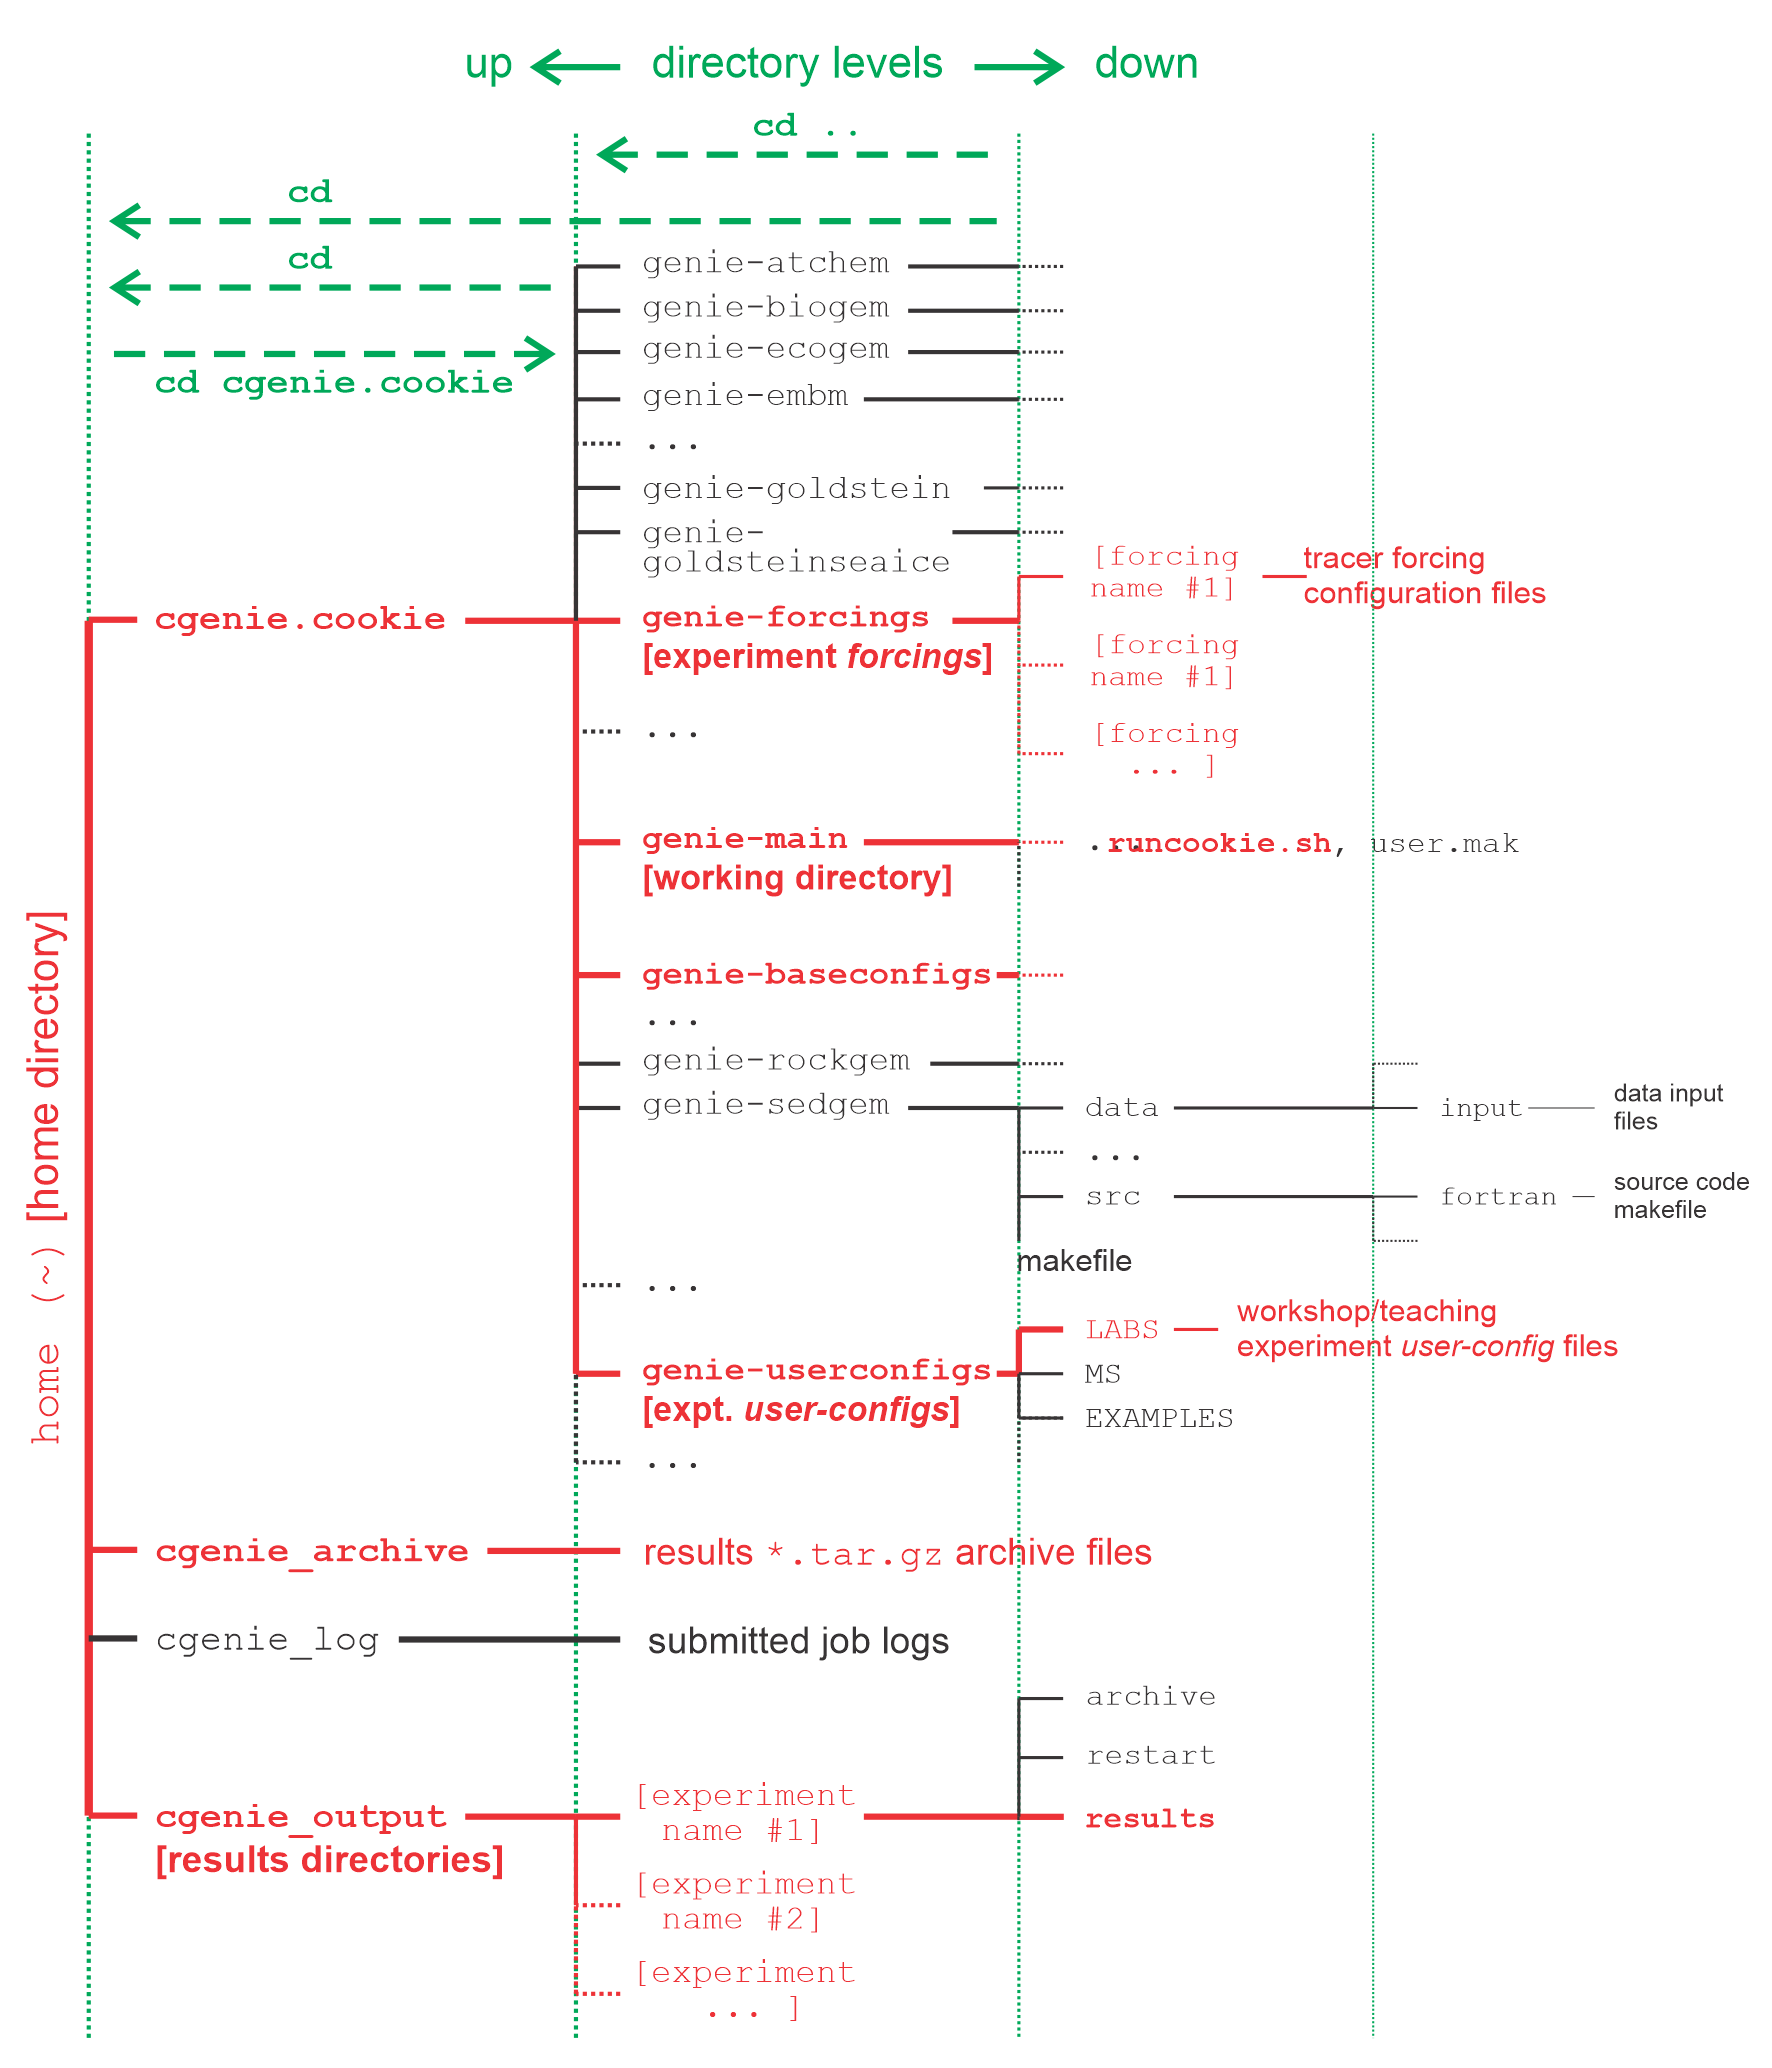
\includegraphics[width=\linewidth]{Figures.usermanual.1.png}
\caption{Directory structure of the \textbf{cookie} model. Highlighted in \textcolor{red}{red} are directories and sub-directories that you will need to access at some point. Vertical \textcolor[rgb]{0,0.501961,0}{green} lines designate directory levels, with example commands shown for moving between them.}
\label{fig:directories}
\end{figure}

%------------------------------------------------
\newpage
%------------------------------------------------

\section{Running the model}

The overall sequence of configuring and running \textbf{cookie} (job submission to a cluster queue), is shown in Figure \ref{fig:chx-jobcreation}. Refer to this if in any doubt at any point.

At the command-line (\texttt{\$}) and \uline{in the \textsf{\footnotesize genie-main} directory} (not your home directory), you will be entering in a command (\texttt{./runcookie.sh}) together with a list of parameters that will be passed to the model, and as if by magic the model will run (or sometimes not). The form of the command you are going to be issuing is:

\vspace{-1mm}\begin{verbatim}
$ ./runcookie.sh #1 #2 #3 #4 (#5)
\end{verbatim}\vspace{-1mm}

\noindent(\uline{don't type it yet}!) It requires that you must list at least 4 parameters after \texttt{./runcookie.sh}, separated by S P A C E S and on a single continuous line (even if it ‘wraps’ around across 2 lines of the screen).
These parameters are:

\vspace{2mm}
\begin{enumerate}[noitemsep]
\setlength{\itemindent}{.2in}
\item[\textbf{\#1}] ... is the name of the required base (or ‘basic’) configuration (‘\textit{base-config}’) of the model.
\item[\textbf{\#2}] ... is the name of the subdirectory (if any) containing the user configuration (‘\textit{user-config}’) file (i.e., the file containing the specification of a particular experiment).
\item[\textbf{\#3}] ... is the name of the experiment itself. There must exist a file in the directory specified by parameter \#2 (\texttt{LABS}) with exactly the same name as you enter here for parameter \#3 (i.e. parameter \#3 points to a file in the directory given by parameter \#2).
\item[\textbf{\#4}] ... is the run length of the experiment in years – this must be entered as an integer.
\item[\textbf{(\#5)}] ... There is also one optional (5th) parameter (to be described later).
\end{enumerate}

%------------------------------------------------
\vspace{1mm}\noindent\rule{4cm}{0.5pt}\vspace{2mm}
%------------------------------------------------

\noindent As an example of running the \textbf{cookie} Earth system model:

\vspace{2mm}
\begin{enumerate}[noitemsep]
\setlength{\itemindent}{.2in}
\item[\textbf{\#1}]: The \textit{base-config} is: \texttt{cookie.CB.p\_worbe2.BASES}
\item[\textbf{\#2}]: The \textit{user-config} directory is: \textsf{\small LABS}
\item[\textbf{\#3}]: The \textit{user-config} file (the experiment name) is: \texttt{LAB.0.3.EXAMPLE}.
\item[\textbf{\#4}]: Run the experiment for ten years: 10
\item[\textbf{\#5}]: (There is no restart file, and so no 5th parameter needs to be passed …)
\end{enumerate}

The full command for your first example experiment, which you are going to issue from the \texttt{\~}\texttt{/cgenie.cookie/genie-main} directory, then looks like:

\vspace{-1mm}\begin{verbatim}
$ ./runcookie.sh cookie.CB.p_worbe2.BASES LABS LAB.0.3.EXAMPLE 10
\end{verbatim}\vspace{-1mm}

\noindent(\uline{you can try it now}!)

\vspace{2mm}
\textbf{REMEMBER: This must be entered on a single CONTINUOUS LINE.}

\textbf{The (single) S P A C E S are vital. }

\textbf{ALSO -- take care not to confuse an el (‘\texttt{l}’) with a one (‘\texttt{1}’)  ... (it is a ‘one’ here).}

%------------------------------------------------
\newpage
%------------------------------------------------

\noindent What should happen is: First, you will end up twiddling your thumbs a while, as all the components of \textbf{cookie} are compiled from the raw source code (\textbf{FORTRAN}). When it has finished doing this, the model will initialize and carry out some brief self-checking. Only then will it start actually ‘running’ and doing something ... in this particular example, the output should look something like this:

\vspace{-2mm}\tiny\begin{verbatim}

 *******************************************************
  *** Initialisation complete: simulation starting ...
 *******************************************************

 >   model year |   pCO2(uatm)   SAT(oC) |   AMOC(Sv)    ice(%)   SST(oC)  SSS(PSU) |       pH  OHMEGA |   [O2](uM)  fPOC(PgC/yr)

 >          0.5 |      285.042    -3.667 |     12.715     0.274     1.408    34.902 |    8.048   2.537 |    181.360        12.327
 >          1.5 |      295.295    -2.531 |     13.189     2.126     3.450    34.902 |    8.079   2.896 |    191.671        12.636
 >          2.5 |      302.383    -1.270 |     12.266     4.282     5.004    34.904 |    8.088   3.131 |    196.879        12.394
 >          3.5 |      307.657    -0.274 |     11.020     5.525     6.214    34.906 |    8.093   3.318 |    199.930        12.216
 >          4.5 |      311.667     0.628 |      9.831     6.037     7.185    34.908 |    8.096   3.469 |    201.861        12.096
 >          5.5 |      314.811     1.437 |      8.876     6.387     7.987    34.910 |    8.099   3.597 |    203.157        11.994
 >          6.5 |      317.299     2.150 |      8.091     6.628     8.667    34.911 |    8.101   3.707 |    204.047        11.899
 >          7.5 |      319.290     2.782 |      7.872     6.673     9.256    34.913 |    8.103   3.800 |    204.669        11.822
 >          8.5 |      320.852     3.342 |      7.886     6.734     9.773    34.914 |    8.105   3.882 |    205.073        11.742
 >>> SAVING BIOGEM TIME-SLICE AVERAGE CENTERED @ year  :        9.500
 >          9.5 |      322.066     3.848 |      7.935     6.684    10.232    34.914 |    8.106   3.954 |    205.320        11.670

 *******************************************************
  *** Simulation complete: shutdown starting ...
 *******************************************************

\end{verbatim}\normalsize\vspace{-2mm}

(Note that you might want to increase the width of your terminal window in order to get the values reported for each year appearing on the same line and not wrapped-over to the next one.)

%------------------------------------------------
\vspace{1mm}\noindent\rule{4cm}{0.5pt}\vspace{2mm}
%------------------------------------------------

\noindent What do all these numbers mean? From left-to-right:

\vspace{1mm}\begin{itemize}
\item[] \texttt{model year}  -- ... guess!
\end{itemize}\vspace{1mm}

\noindent Then:

\vspace{1mm}\begin{itemize}
\item[] p\(CO_{2}\)(uatm) -– mean atmospheric CO\(_{2}\) concentration (in units of \(\mu\)atm)
\item[] \texttt{<SST>} -- global mean surface air temperature ('SAT') $^{\circ}$C
\end{itemize}\vspace{1mm}

Note that if you are not running an experiment without a carbon cycle, there will be no values for p\(CO_{2}\).

\vspace{1mm}\begin{itemize}
\item[] \texttt{AMO(Sv)} -- Atlantic meridional overturning circulation (AMOC) (Sv)
\item[] \texttt{ice(\%)} -- global sea-ice fraction (\%)
\item[] \texttt{<SST>} -- global sea surface temperature ('SST') $^{\circ}$C
\item[] \texttt{<SSS>} -- global sea surface salinity ‘SSS’ (\%\textit{o})
\end{itemize}\vspace{1mm}

Note that if you are not running an experiment with a modern-like Atlantic basin, no value is given for the AMOC.

\vspace{1mm}
\noindent After that, a couple of carbonate chemistry indicators:

\vspace{1mm}\begin{itemize}
\item[] \texttt{pH} -- Mean ocean surface pH.
\item[] \texttt{OHMEGA} -- Mean ocean surface OHMEGA ...
\end{itemize}\vspace{1mm}

\noindent which will become apparent later.

Note that if you are not running an experiment without a carbon cycle, no values will be given.

%------------------------------------------------
\newpage
%------------------------------------------------

\noindent Finally:

\vspace{1mm}\begin{itemize}
\item[] \texttt{O2} -- Dissolved oxygen in the ocean(global mean). ($\mu mol kg^{-1}$)
\item[] \texttt{fPOC} -- Global total annual export production (in terms of particulate organic carbon ($PgC yr^{-1}$).
\end{itemize}\vspace{1mm}

Note that you need some sort of biological pump in the ocean for these to be meaningful.

%------------------------------------------------
\vspace{1mm}\noindent\rule{4cm}{0.5pt}\vspace{2mm}
%------------------------------------------------

\noindent The choice of what information to display on screen as the model is running is rather arbitrary, but the chosen metrics do tend to summarize some of the main properties of the climate system and carbon cycle – for my own personal convenience rather than reflecting any fundamental scientific truth ... 

This information is reported at the same intervals as \textit{time-series} data (see later and/or refer to the User Manual) is saved and is indicated by:

Interleaved between these lines are lines reporting the saving of \textit{time-slice} data (the 2- and 3-D model states – more of which later as well as in the User Manual). These appear as:

\vspace{-2mm}\small\begin{verbatim}
>>> SAVING BIOGEM TIME-SLICE AVERAGE CENTERED @ year:
\end{verbatim}\normalsize\vspace{-2mm}

\noindent \textbf{You can stop the model at any point (all data up to that time will have been saved) by hitting: \textsf{\footnotesize <Ctrl-C>} (\textsf{\footnotesize CONTROL} key + ‘\textsf{\footnotesize C}’ key).}

%------------------------------------------------
\vspace{1mm}\noindent\rule{4cm}{0.5pt}\vspace{2mm}
%------------------------------------------------

\noindent Just from examining the screen output: how close to steady state does the system appear to have come after just 10 years? i.e., do SST and/or sea-ice extents appear to be converging towards stable (constant) values? This will be an important question to think about later on: ‘has the model reached steady-state (and does it matter)?’

%------------------------------------------------
\vspace{1mm}\noindent\rule{4cm}{0.5pt}\vspace{2mm}
%------------------------------------------------

\begin{figure}
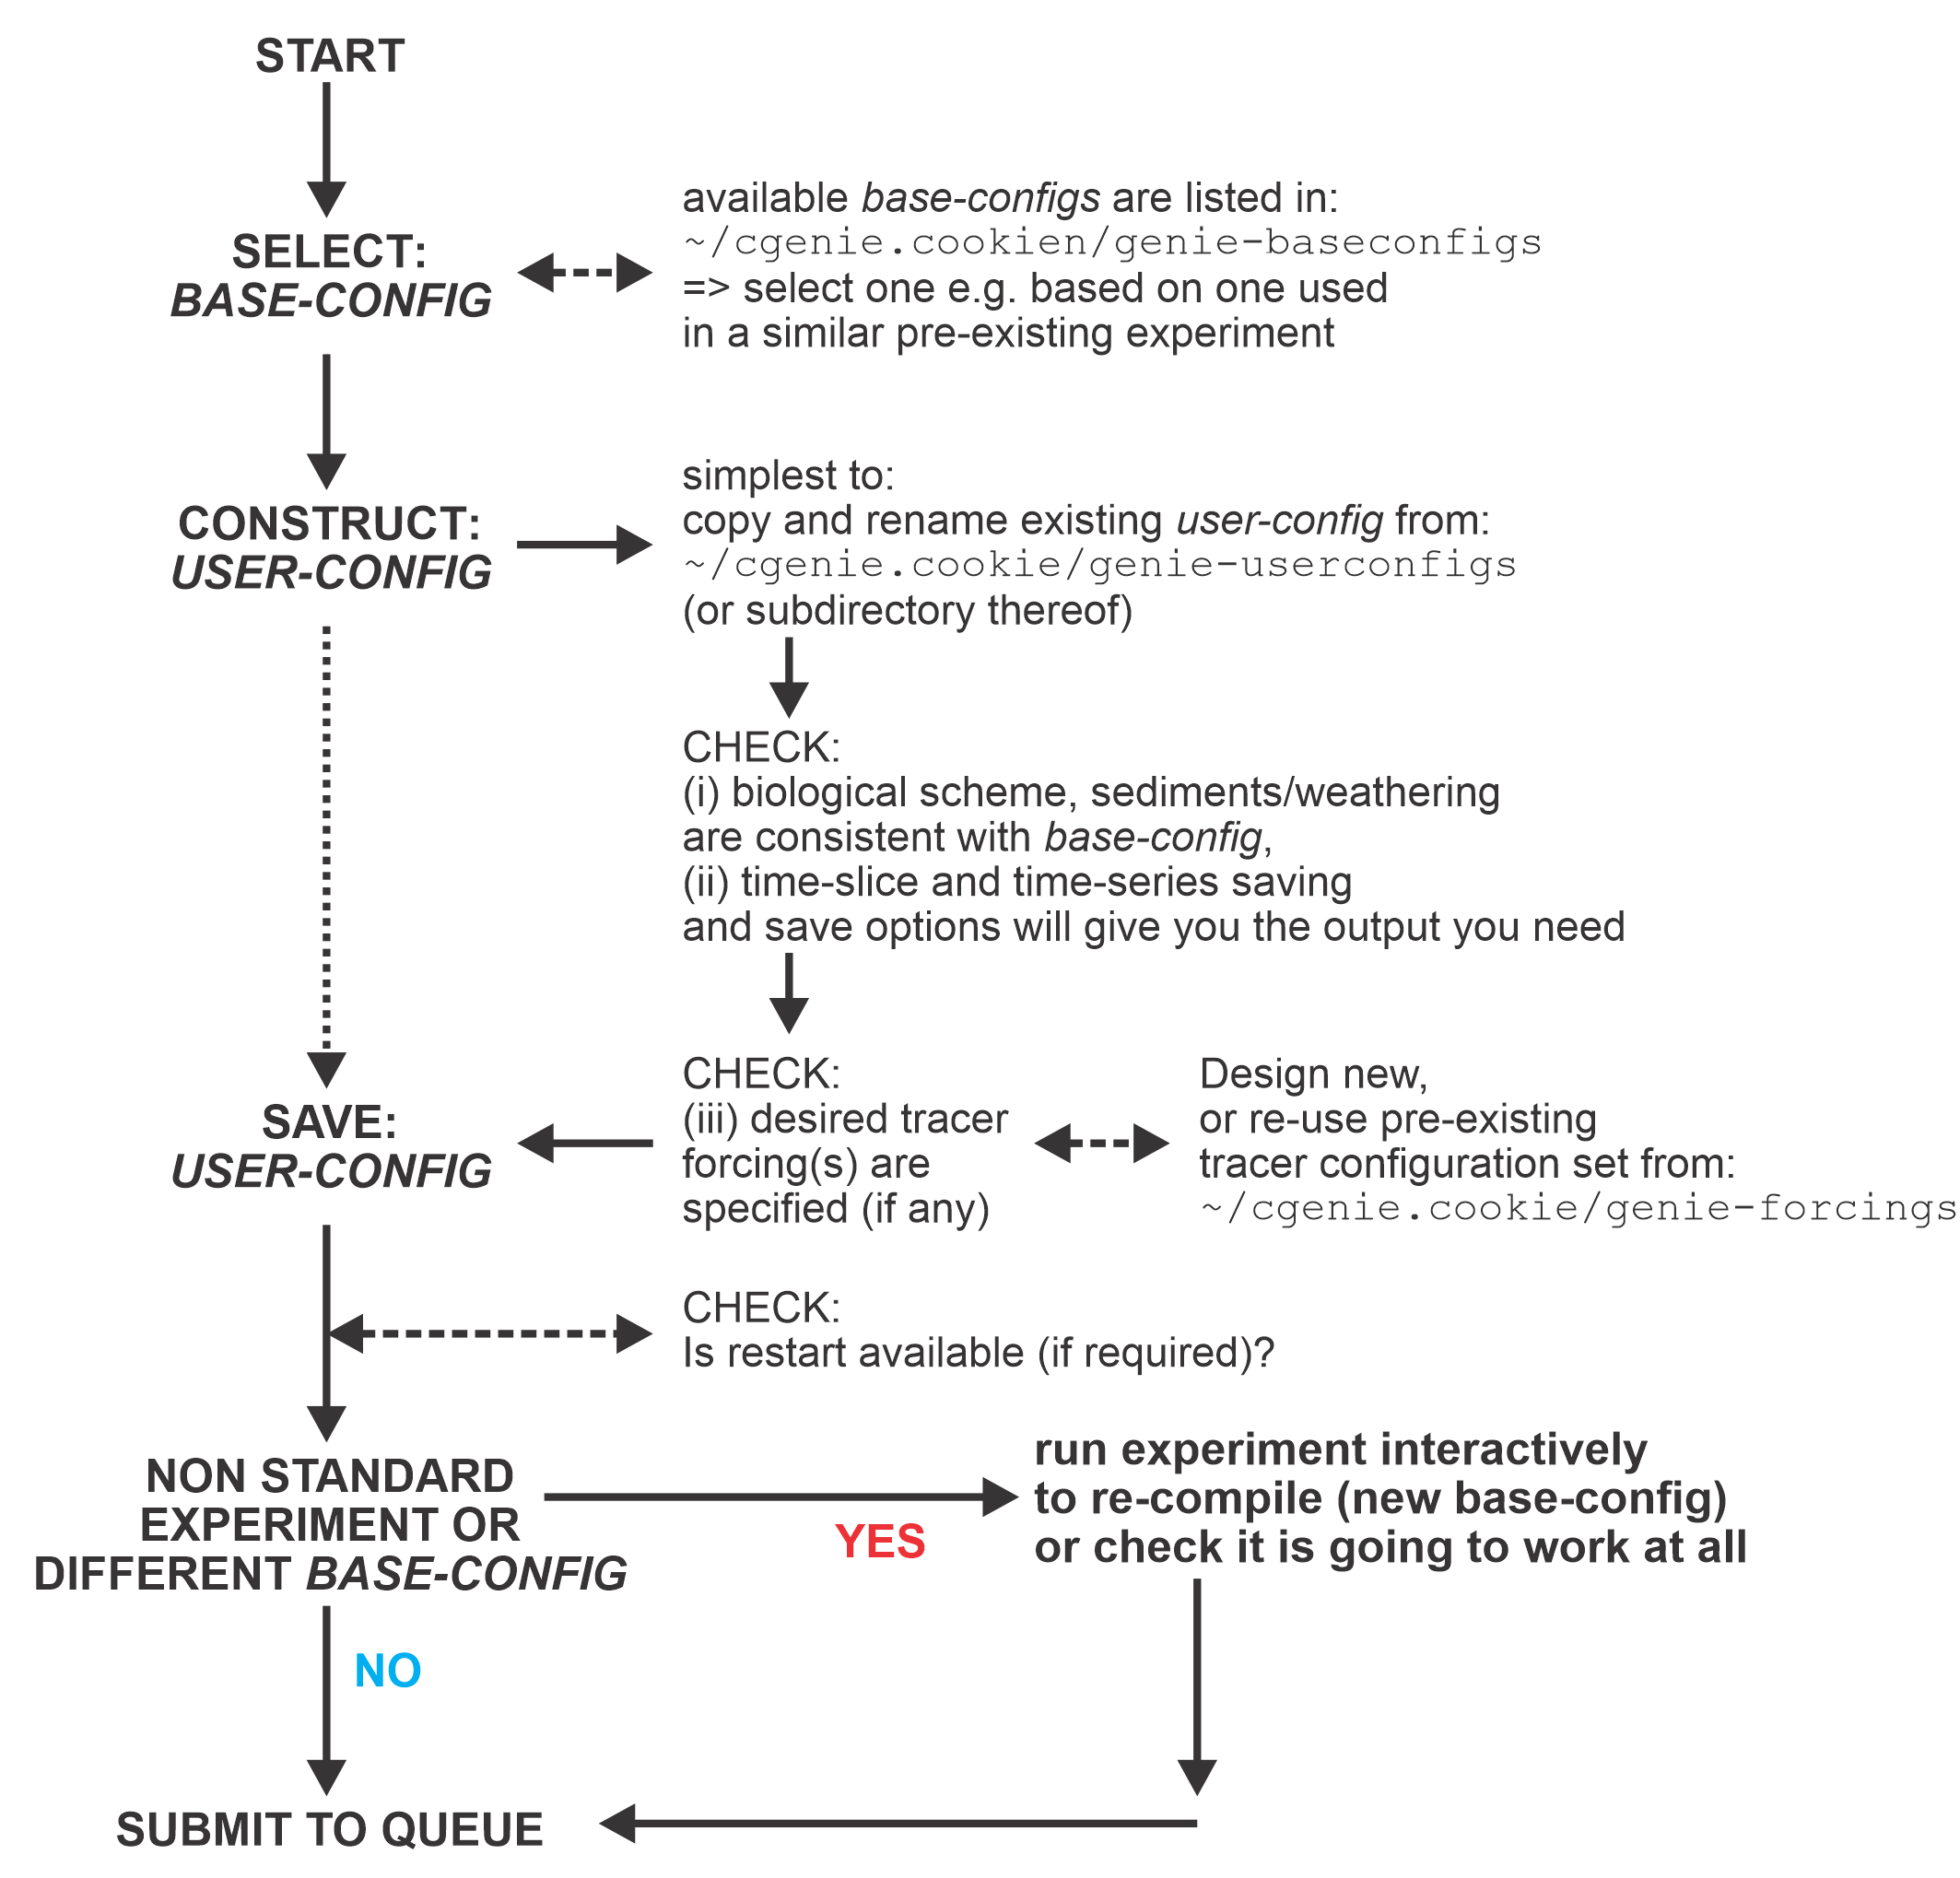
\includegraphics[width=0.8\textwidth]{Figures.usermanual.2.png}\centering
\vspace{2mm}
\caption{Schematic of the sequence-of-events in configuring and running an experiment.}
\label{fig:chx-jobcreation}
\end{figure}

%------------------------------------------------
\newpage
%------------------------------------------------

\section{Creating new experiments!}

The key to creating new experiments is to \textbf{remember that the name of the \textit{user-config} file, that contains the parameter settings that define that specific experiment, becomes the name of the experiment and hence name of the model results sub-directory in \textsf{\footnotesize cgenie\_output}}. Changing the name of the \textit{user-config} file, hence leads to a new experiment name and a new model results sub-directory. (Conversely, not changing the name of the  \textit{user-config} file and re-running it results in the results of any previous experiment run using that \textit{user-config} file, being over-written.)

There are two obvious ways to create a new \textit{user-config} file and hence new experiment:

\begin{enumerate}[noitemsep]

\vspace{1mm}
\item Create a blank text file \footnote{\texttt{\$ touch file.txt} will achieve this at the linux command line.} and populate the contents with the parameter value assignments you need for your new experiment.
\\Inevitably, it is difficult to remember all the names and even values you want to specify, meaning that you'll end up looking at existing \textit{user-config} files and copying and pasting lines (or even the entire contents) from the old file(s) into your new \textit{user-config} file. So then you may was well ...

\vspace{1mm}
\item Copy and edit an existing file!
\\This is the most practical approach -- pick an existing \textit{user-config} file that is closest to the specific experiment that you want to run -- copy and rename it, then edit the contents and save. For the purpose of trying this out, you can literally pick on any existing file in the \textsf{\footnotesize LABS } subdirectory (of \textsf{\footnotesize genie-userconfigs}).
\vspace{1mm}
\\ You can do this by:
\begin{itemize}[noitemsep]
\vspace{1mm}
\item Using your sftp client (program):
\\First -- drag the existing \textit{user-config} file to your local computer. On your local computer, rename the file as per how you would 'normally' rename any file. 
\\Now you can edit the parameter values, re-save it, drag it back to the cluster (from your local computer) using the sftp client ... and finally run the experiment.
\\There are also ways of configuring \textbf{sftp} clients so that you can double-click on a file in the remove window, edit it, and save it back to the remote computer.\footnote{Actually what happens is that the file is transferred locally, opened, and you edit a local copy. When you save it (locally), it is automatically transferred back.} 
\vspace{1mm}
\item Or, if you are comfortable working at the linux command line; working from the same directory (e.g. \textsf{\footnotesize LABS}) that the file you want to copy lives in, you can copy a file (to a new filename) by:
\\\texttt{\$ cp oldfile newfile }
\\(after which you can edit the new \textit{user-config} file \textsf{\footnotesize newfile}, re-save, and then run the experiment.)
\end{itemize}
\vspace{1mm}

\end{enumerate}

\noindent Remember that the new \textit{user-config} file needs to be saved in (or copied to) the \textsf{\footnotesize genie-userconfigs/LABS} sub-directory (in the case of experiments carried out as part of the tutorials described in this manual), or \textsf{\footnotesize LABS} itself or any sub-directory (or sub-sub- etc directory) ... as long as you specify the correct path to the directory where you save the new file to\footnote{See previous Section and the use of the 2nd parameter passed to \texttt{runcookie.sh}}.

%------------------------------------------------
\newpage
%------------------------------------------------

\section{Model output}

Experiment results are saved in a single sub-directory of the experiment results directory (along with a sub-directory for \textit{restart} files, and one for copies of your parameter choices). The directories continaing the results of all your different experiment live in:

\vspace{-1mm}\begin{verbatim}
~/cgenie_output
\end{verbatim}\vspace{-1mm}
and will be assigned a directory name something like:

\vspace{-1mm}\begin{verbatim}
LAB.0.3.EXAMPLE
\end{verbatim}\vspace{-1mm}
(this being the results directory name for an experiment called \textsf{\footnotesize LAB.0.3.EXAMPLE}) and the actual results results live in a sub-directory of this -- \textsf{\footnotesize results}, hence:

\vspace{-1mm}\begin{verbatim}
~/cgenie_output/LAB.0.3.EXAMPLE/results
\end{verbatim}\vspace{-1mm}

\noindent NOTE: If in an sftp client window you find that you cannot 'see' the \textsf{\footnotesize cgenie\_output} directory ... or cannot find any of the results sub-directories you are expecting, \uline{you will need to refresh the directory listing} (e.g. for \textbf{WinSCP}, there is a double green-arrow \textsf{\footnotesize Refresh} icon button near the top right of the window that you can click on). sftp client programs generally do not automatically refresh directory listing on the remote computer.

%------------------------------------------------
\vspace{1mm}\noindent\rule{4cm}{0.5pt}\vspace{2mm}
%------------------------------------------------

\noindent \textbf{cGENIE.cookie} has a flexible and powerful facility of saving results by means of spatially explicit ‘time-slices’, and as a semi-continuous ‘time-series’ of a single global (or otherwise representative mean) variable, described as follows.

%------------------------------------------------

\subsection{Time-slice output}

One of the most informative data sets that can be saved is that of the spatial distribution of properties (such as tracers or physical ocean attributes). However, saving full spatial distributions (e.g., a 36\(\times\)36\(\times\)8 array) for any or all of the tracers each and every time-step is clearly not practical; not only in terms of data storage but also because of the detrimental effect that repeated file access has on model run-time.
Instead, \textbf{BIOGEM} will save the full spatial distribution of tracer properties only at one or more predefined time points (in units of years). These are termed \textit{time-slices}. At the specified time points, a set of spatially-explicit data fields are saved for all the key tracer, flux, and physical characteristics of the system. However, rather than taking an instantaneous snapshot, the time-slice is constructed as an average over a specified integration interval (the default is set to 1.0 years, i.e. an annual average). \textbf{BIOGEM}  assumes that the specified time point represents the mid-point of the (annual) average with the results that output years end up being reported.

\vspace{1mm}
For example, to save regularly every 10 years you would set:

\vspace{-1mm}
\small\begin{verbatim}
bg_par_data_save_slice_timeinterval=10.0
\end{verbatim}\normalsize
\vspace{-1mm}
and which would give you save points at:

\vspace{-1mm}\footnotesize\begin{verbatim}
9.5
19.5
29.5
39.5
…
\end{verbatim}\normalsize\vspace{-1mm}
(the mid-points of averages made over the intervals: 9-10, 19-20, 29-30, 39-40 years, etc.).

\noindent Otherwise, you can specify the name of a file containing times to save at, or simply only save at the end. (see later)

%------------------------------------------------
\newpage
%------------------------------------------------

\subsection{Time-series output}

The second data format for model output is much more closely spaced in time. Model characteristics must then be reducible to a single meaningful variable for this to be practical (i.e., saving the time-varying nature of 3-D ocean tracer distributions is not). Suitable reduced indicators would be the total inventories in the ocean and/or atmosphere of various tracers (or equivalently, the mean global concentrations / partial pressures, respectively). Like the time-slices, the data values saved in the time-series files represent averages over a specified integration interval (the default is set to 1.0 years (annual average) but the results are reported with respect to the mid-point of the average which is where the ‘.5’ bits come in again).

The much smaller and simpler (text) file format now allow you to save much more frequently. For example, for experiments up to a few 100 years, you could save every single year, which you would set by:

\vspace{-1mm}
\small\begin{verbatim}
bg_par_data_save_sig_timeinterval=1.0
\end{verbatim}\normalsize
\vspace{-1mm}

\noindent Otherwise, you can specify the name of a file containing times to save at. (see later)

%------------------------------------------------

\subsection{File naming convention}

The \textsf{\footnotesize results} results directory will contain files with names of the form:

\vspace{1mm}
\begin{itemize}[noitemsep]
\setlength{\itemindent}{.2in}
\item \textsf{\footnotesize fields\_biogem\_2d.nc} – 2-D fields of ocean and atmosphere properties, as \textbf{NetCDF}.
\item \textsf{\footnotesize fields\_biogem\_3d.nc} – 3-D fields of ocean properties, as \textbf{NetCDF}.
\item \textsf{\footnotesize timeseries\_*.txt} – these are the time-series files (in ASCII / plain text format).
\item \textsf{\footnotesize SUMMARY\_AT\_year\_*\_diag\_GLOBAL.txt} – these contain (global diagnostics) summary information and are saved at the same frequency as the time-slices (also as ASCII / plain text).
\end{itemize}
\vspace{1mm}

%------------------------------------------------
\vspace{1mm}
\noindent\rule{4cm}{0.1mm}
%------------------------------------------------

\subsection*{Alternative file naming convention ...}

Having the e.g., 2D and 3D \textbf{netCDF} files always called the same name (\textsf{\footnotesize fields\_biogem\_2d.nc}, \textsf{\footnotesize fields\_biogem\_3d.nc}) in each and every experiment, has the potentil to get confusing if you have multiple experiments open simultaneously in a viewer such as \textbf{Panoply}.

You can specify that \textbf{netCDF} files are named following the name of your experiment, by adding the following line to your \textit{user-config}:

\vspace{-1mm}\begin{verbatim}
bg_ctrl_ncout_expid_name=.true.
\end{verbatim}

%------------------------------------------------
\newpage
%------------------------------------------------

\section{Viewing model output}

%------------------------------------------------

\subsection{Time-series output}

A descriptive summary of all the time-series (\textsf{\footnotesize biogem\_series\_*.res}) data files is given in the \textbf{cookie} User Manual if you are really that bored. The files of most immediate use/relevance are:

\vspace{1mm}
\begin{itemize}[noitemsep]
\setlength{\itemindent}{.2in}
\item \textsf{\footnotesize timeseries\_atm\_humidity.res}  - mean atmospheric (surface) humidity
\item \textsf{\footnotesize timeseries\_atm\_temp.res}      - mean atmospheric (surface) air temperature
\item \textsf{\footnotesize timeseries\_misc\_opsi.res}     - overturning stream-function (e.g. AMOC) strength
\item \textsf{\footnotesize timeseries\_misc\_seaice.res}   - mean ocean sea-ice cover and thickness
\item \textsf{\footnotesize timeseries\_ocn\_sal.res}       - mean ocean surface and whole ocean salinity
\item \textsf{\footnotesize timeseries\_ocn\_temp.res}      - mean ocean surface and whole ocean temperature
\end{itemize}

%------------------------------------------------
\vspace{1mm}\noindent\rule{4cm}{0.1mm}\vspace{2mm}
%------------------------------------------------

\noindent One way of viewing the contents of files (in a shell window/terminal) is to change directory to the experiment results directory and opening the file in a file editor at the command line. But that is not so much fun.

Instead – change to the experiment results directory and then to the \textsf{\footnotesize biogem} sub-directory in the Secure File Transfer Client, and try double-clicking (if you have set up the \textbf{WinSCP} preferences correctly) or right-mouse-button-clicking (the then Edit with) on one of the .res files (listed above).
\vspace{1mm}
For \texttt{timeseries\_ocn\_temp.txt}, you should see 5 columns:
\small\begin{verbatim}
 % time (yr) / temperature (C) / _surT (ice-free) (C) / _benT (C) / _surT (C)
\end{verbatim}\normalsize
for: model time (years) (actually, the mid-point in time of an annual average), annual mean ocean temperature (averaging over the entire ocean volume), annual mean ocean surface temperature (excluding ice-cover areas), annual mean benthic (sea-floor) temperature, annual mean ocean surface temperature (now including ice-cover areas). Other results files may differ in the numbers of columns but all should be identifiable from the header (first line) information.

Remember: \textbf{WinSCP} does not automatically refresh the directory listing. If you cannot see the results sub-directory with the experiment name you have just run, 99 times out of 100, it is because the display of the \textbf{WinSCP} needs to be refreshed -- there is an icon at the top of the program window or hit the ‘\textsf{\footnotesize F5}’ key.

\vspace{1mm}
\noindent\rule{4cm}{0.1mm}
\vspace{2mm}

\noindent For your information and edification (only): \textbf{Excel}, or \textbf{MUTLAB} if you prefer, can be used to graph the time-series results. Either way you will have to deal with the header line(s) that are present at the top of the file (and preceding the rows of data).

In \textbf{Excel}: Choose \textsf{\footnotesize File} then \textsf{\footnotesize Open}.  You will want to select \textsf{\footnotesize Files of Type} ‘\textsf{\footnotesize All Files (*.*)}’. In the \textsf{\footnotesize Text Import Wizard} window you can request that \textbf{Excel} skips the first few lines to start the import on the 2nd or 3rd line of the text file. Alternatively: set an appropriate column width manually in \textbf{Excel} to ensure that the columns of data are correctly imported.

\textbf{MUTLAB} will ignore lines starting with a \textsf{\footnotesize \%}, which the time-series starts with. However, it may be that the header line wraps-around and there is in effect a 2nd header line but without a \textsf{\footnotesize \%}. In this case, extra care (or a quick edit of the header in the ASCII file) will be required to load the data into \textbf{MUTLAB}.

%------------------------------------------------
\newpage
%------------------------------------------------

\subsection{2- and 3-D time-slice output}

For the time-slice \textbf{NetCDF} (*.nc) files you will be using a program called \textbf{Panoply}. If you want your own (FREE!) copy of this utility, you can get it here (and is available for: \textbf{Windoz}, \textbf{Mac}, and linux operating systems): http://www.giss.nasa.gov/tools/panoply/.

\vspace{1mm}

\noindent When you open the \textbf{NetCDF} file, you will be presented with a ‘\textsf{\footnotesize Datasets and Variables}’ window (on the left hand side of the application window). This contains a list of all the parameters available that you can display. You will find that the ‘\textsf{\footnotesize Long Name}’ description of the variable will be the most helpful to identify the one you want. Simply double-click on a variable to display. 

For the 3-D fields you will be asked first whether you want a ‘\textsf{\footnotesize \footnotesize Longitude-Latitude}’ or ‘\textsf{\footnotesize Latitude-Vertical}’ plot (for the 2-D fields, the plot display will immediately open).
For the ‘\textsf{\footnotesize Longitude-Latitude}’ plots – there are multiple levels (depth layers) in the ocean - these data that can be plotted from the surface to the abyssal ocean. For the ‘\textsf{\footnotesize Latitude-Vertical}' plots – there are multiple possible longitudes at which to plot slices. The default is the global mean meridional distribution. There is also an option for ‘\textsf{\footnotesize Longitude-Vertical}' plots (which we will not use).

There may be multiple time-slices (i.e., you can plot data saved from different years). By default, only the very first \textit{time-slice} will be displayed.

You can choose interpolate the data or not (often you may find that it is clearer not to interpolate the data but to leave it as ‘blocky’ colors corresponding to the resolution of the model), change the scale and colors, overlay continental outline, change the projection, etc etc. Grey cells represent ‘dry’ grid points, i.e., continental or oceanic crust.

\vspace{1mm}
NOTE: The default settings in \textbf{Panoply} can mislead. Be aware of:
\vspace{1mm}
\begin{enumerate}
\item \textbf{Panoply} initially displays the very 1st time-slice (often year mid-point 0.5) time-slice rather than the experiment end. This can confuse and look like an experiment has not done anything!
\item By interpolating the data (not always misleading). To remove interpolation, un-tick:
\\‘\textsf{\footnotesize Interpolate}’ in the ‘\textsf{\footnotesize Arrays}’ tab.
\item By displaying a global zonal mean by default when selecting \textsf{\footnotesize Latitude-Vertical} plots. Then, to further confuse you, by plotting the output up-side-down (to invert: in the ‘\textsf{\footnotesize Grid}’ tab, hit ‘\textsf{\footnotesize Swap B/T}’ (for swap bottom/top).
\item By listing all ‘\textsf{\footnotesize Plottable variables}’ (option at the bottom of the window), when what you \textit{ideally} want are  the shorter and less confusing list of ‘\textsf{\footnotesize Georeferenced variables}’.
\item In \textsf{\footnotesize Longitude-Latitude} plots, by overlaying the modern continental output. (\textbf{cookie} land is marked in grey.)
\item By fitting a scale to the plot when the display window is opened, but not changing the scale when e.g., time or depth is changed. (The point of confusion is that you can quickly move outside the scale and end up with all model points dark blue or red.) Re-fit the scale, or manually set limited, in the ‘\textsf{\footnotesize Scale}’ tab.
So be careful when opening a new plot that you are looking at what you *think* you are looking at …
All the defaults can be changed via the ‘\textsf{\footnotesize Edit}’ drop-down menu and ‘\textsf{\footnotesize Preferences}’.
\end{enumerate}

%------------------------------------------------
\vspace{1mm}\noindent\rule{4cm}{0.1mm}\vspace{2mm}
%------------------------------------------------

\noindent To save plots in \textbf{Panoply}:
\footnotesize
\\\textsf{File}
\\\textsf{Save Image As …}
\normalsize
\\Then select the location, filename, and graphics format.

%------------------------------------------------
\newpage
%------------------------------------------------

\section{Submitting experiment ‘jobs’}

This bit is no particular fun at all, but it is a very handy ‘trick’ for running the model in the background, and maximizes drinking time in the bar vs. sat bored watching a computer screen :)

%------------------------------------------------
\vspace{1mm}\noindent\rule{4cm}{0.1mm}\vspace{2mm}
%------------------------------------------------

\noindent Running jobs interactively is all very well, but there are three important limitations:
\begin{enumerate}[noitemsep]
\vspace{1mm}
\item The connection between your terminal and the server computer running the model must remain unbroken. Anything more than a fleeting loss of internet connectively may result in the experiment terminating.
\vspace{1mm}
\item You can only run one experiment at a time … unless you want to have thousands of separate terminal open …? I thought not …
\vspace{1mm}
\item Any cluster or computer you are likely to be accessing using a shell will not have many computing cores itself, either because it is a single machine with only one or two processors, or if a cluster, by using a terminal you are running on the ‘head node’, which will have similar computing core limitations to running on a single machine. The more experiments you run simultaneously, the slower they will all run …
\end{enumerate}

%------------------------------------------------
\vspace{1mm}\noindent\rule{4cm}{0.1mm}\vspace{2mm}
%------------------------------------------------

\noindent The alternative is to submit your experiment as a ‘job’ to a queuing system which then manages what compute resources are used to run the model. Once you have submitted the experiment, that is it – you can go straight to the bar :)

For example -- to run the same experiment as before (\textsf{\footnotesize LAB\_0.EXAMPLE}) for maybe 100 years (or even longer if you wish – I am just pulling factors of 10 out of thin air here) but now submit the experiment as a job to the cluster queue, type (again: SINGLE, CONTINUOUS LINE):
\vspace{-1mm}
\small\begin{verbatim}
$ qsub -q QUEUE.q -j y -o cgenie_log -V -S /bin/bash runcookie.sh
  ./runcookie.sh cookie.CB.p_worbe2.BASES LABS LAB.0.3.EXAMPLE 100
\end{verbatim}\normalsize
\vspace{-1mm}

Here, the queue name for this\ particular cluster is \textsf{\footnotesize QUEUE.q}. \uline{The cluster you are actually using will have a different queue name} (e.g. refer to any cluster-specific information that you might have).

\vspace{1mm}
Note that now you should omit the ‘\texttt{./}’ bit before \texttt{runcookie.sh}.
(If you are interested (I know that you are not): the options following \texttt{qsub} and before \texttt{runcookie.sh} do things like re-directing screen output and error messaging to a file and specify which linux ‘shell’ to assume. It is even possible to receive an email when the job is done :) )
The status of the cluster queue and how you experiment job is getting on (e.g., “Is it finished yet?”) can be checked by typing:
\vspace{-1mm}
\small\begin{verbatim}
$ qstat -f
\end{verbatim}\normalsize
\vspace{-1mm}
(\texttt{qstat -f -u "*"} will show all jobs on the cluster.)

\vspace{1mm}
After submitting an experiment, you receive a job number. This number appears in the first column in the queue status information when you issue a qstat –f command. You should see your job appear on one of a number of compute nodes, perhaps numbered 0-0 through 0-5), although it might briefly reside as a ‘\textsf{\footnotesize PENDING JOB}’. For each node, there are multiple processing cores (depending on the specific cluster and queue), meaning that multiple instances of \textbf{cookie} can run simultaneously on each node. For an 8-level ocean based configuration of \textbf{cookie}, being run for 100 years, the job should remain there in the queue for a few minutes before ‘disappearing’ (your clue that it has finished, or died\footnote{If your experiment appears on the queue but vanishes after a few seconds, it has most likely died :(} …). If you periodically re-issue a \texttt{qstat –f} command you can follow your job’s progress.

A rough rule of thumb is that 8-level ocean \textbf{cookie} @ a horizontal grid resolution of 36x36 will simulate about 1000 years per CPU hour. The 16-level version (which you will use later), runs at about 300-400 years per CPU hour.

\vspace{1mm}
\noindent \textbf{NOTE}: It may be that the \textbf{FORTRAN} compiler is not accessible by the computer nodes. The implication of this is that \textit{the \textbf{cookie} executable must be already compiled BEFORE a job is submitted to the queue}. In other words; if you have just changed the model resolution or continental configuration, or number of tracers (i.e. changed the \textit{base-config}) or issued a \texttt{make cleanall} command you MUST briefly run your desired experiment (or equivalent) interactively (i.e., in the shell window) to ensure that everything is correctly compiled. For instance, either run the experiment for a couple of years or start the experiment for the desired full duration, but 'kill it' (\textsf{\small Ctrl-C}) once the experiment is running successfully.

%------------------------------------------------
\newpage
%------------------------------------------------

\section{‘Restarts’}

Not much fun here either … but again... an important and time-saving (== increased drinking time!) modelling technique to learn to use.

By default, model experiments start from ‘cold’, i.e., the ocean is at rest and uniform in temperature and salinity while the atmosphere is uniform in temperature and humidity. All biogeochemical tracers in the ocean have uniform concentrations and/or are zero and there are no biogenic materials in deep-sea sediments. From this state it will take several thousand years (kyr) for the climate system to reach steady-state, and closer to 5 kyr (or more) for ocean biogeochemical cycles and atmosphere \(CO_{2}\) to reach steady-state, and exceeding 100 kyr for sediment composition to re-balance weathering ... Reaching this the equilibrium state is called the ‘\textit{spin-up}’ phase of the model.
There is evidently little point in repeating the \textit{spin-up} for each and every model experiment that are similar except in a single detail (e.g., testing a variety of different \(CO_{2}\) emissions scenarios all starting from current year 2012 conditions). A facility is thus provided for requesting that a ‘\textit{re-start}’ is used – starting a new experiment from the end of a previous one, usually a \textit{spin-up} that has been run explicitly for the purpose of generating a starting point (\textit{re-start}) of the system at steady-state (equilibrium) for subsequent experiments to continue on from.
It is important to note that there is nothing special about a \textit{re-start} – it is simply an experiment that you have already run. Equally, there is nothing special about the \textit{re-start}s you will download next – these you could have generated yourself – it simply saves time to have them provided.

\vspace{1mm}
\noindent\rule{4cm}{0.1mm}
\vspace{2mm}

\noindent To experiment with using a \textit{re-start}, you will first need to download a file that has been created (a pre-run 10,000 year spin-up). To fetch this: Change to the \textsf{\footnotesize cgenie\_output} directory (perhaps by going ‘home’ first (\texttt{cd} \textsf{\small <Enter>}), and then changing to \textsf{\footnotesize cgenie\_output} – refer to linux commands HOW-TO and Figure 1.1), and type:

\vspace{-2mm}\small
\begin{verbatim}
$ wget --no-check-certificate http://www.seao2.info/cgenie_output/
   cookie.CB.p_worbe2.BASES.ridgwelletal.SPIN.tar.gz
\end{verbatim}\normalsize
\vspace{-2mm}
(all one line!)

This downloads an archived/compressed copy of the restart from a location on the interweb. Extract the contents of this archive by typing:

\vspace{-2mm}\small
\begin{verbatim}
$ tar xfzv cookie.CB.p_worbe2.BASES.ridgwelletal.SPIN.tar.gz
\end{verbatim}\normalsize
\vspace{-2mm}

Finally, change directory back to \textsf{\footnotesize cgenie.cookie} and then \textsf{\footnotesize genie-main} so that you are ready to run the model (the model is *always* run from the \textsf{\footnotesize cgenie.cookie/genie-main} directory).

\vspace{1mm}
\noindent\rule{4cm}{0.1mm}
\vspace{2mm}

\noindent A \textit{re-start} can be requested for  running on a new experiment from the end of a previous one, by providing a 5th (optional) parameter when entering in the \texttt{runcookie.sh} command. A spin-up of the modern World climate state is provided for you as a \textit{restart} -- 
\textsf{\footnotesize cookie.CB.p\_worbe2.BASES.ridgwelletal.SPIN} -- which you have just unpacked to the \textsf{\footnotesize cgenie\_output} results output directory.

To test out the use this \textit{restart} -- create a new (\textit{user-config}) experiment configuration file in the directory: 

\vspace{1mm}
\textsf{\footnotesize \(\sim\)/cgenie.cookie/genie-userconfigs/LABS}
\vspace{1mm}

\noindent taking the file \textsf{\footnotesize LAB\_0.3.EXAMPLE} (which is provided) as a template (no parameter changes need to be made yet). As described earlier -- copy this file and give it a new name -- here, name it: \textsf{\footnotesize LAB.0.3.NEW}

%------------------------------------------------
\newpage
%------------------------------------------------

\noindent You can then specify the use of the \textit{restart} in your new \textsf{\footnotesize LAB\_0.3.NEW} experiment:

\vspace{-2mm}
\small\begin{verbatim}
$ ./runcookie.sh cookie.CB.p_worbe2.BASES LABS LAB.0.3.NEW 100 
   cookie.CB.p_worbe2.BASES.ridgwelletal.SPIN
\end{verbatim}\normalsize
\vspace{-2mm}

The run-time output should now look noticeably different. There should be no (or perhaps just very little) drift in any of the various variable values outputted to the screen – this is because you have (re-)started from the end of a run that had already ready an equilibrium (or close).

Because \textsf{\footnotesize LAB.0.3.EXAMPLE} (and hence your copy, \textsf{\footnotesize LAB\_0.3.NEW}) does not prescribe a value of $pCO_2$ but instead allows it to 'float', your experiment is a good test of whether the carbon cycle in experiment \\\textsf{\footnotesize cookie.CB.p\_worbe2.BASES.ridgwelletal.SPIN} was at steady state.

%----------------------------------------------------------------------------------------
%----------------------------------------------------------------------------------------